%%%%%%%%%%%%%%%%%%%%%%%%%%%%%%%%%%%%%
%%%%%%%%%%%%%%%%%%%%%%%%%%%%%%%%%%%%%
%
%   Hi, All
%   Arun Xavier, VAST Thrissur
%
%   for more  Visit my Page - http://arunxeee.blogspot.in/
%
%%%%%%%%%%%%%%%%%%%%%%%%%%%%%%%%%%%%
%%%%%%%%%%%%%%%%%%%%%%%%%%%%%%%%%%%%
%
%
%
%******************************************************
%

%%
\documentclass[12 pt, oneside]{book}
\usepackage{graphicx, fancyhdr, amsmath, times,  enumerate,geometry,makeidx,setspace,nomencl,eso-pic,xcolor,lipsum,calc,pst-node,tikz,fancybox,background,caption,subcaption,amsfonts}



\usetikzlibrary{calc}
\SetBgScale{1}
\SetBgAngle{0}
\SetBgColor{brown}
\SetBgOpacity{1}
%%
\geometry{verbose,a4paper,tmargin=1 in,bmargin=1in,lmargin=1.5 in,rmargin=.9 in}
%%%%%%%%%%%%%%%%%%%%%%%%%%%%%%%

\makeindex

%%
\usepackage[final]{pdfpages}
%%
%\setlength{\oddsidemargin}{2 cm}
%%
\newcommand{\VAtitle}[1]%
{\def\vtitle{#1}}%
\newcommand{\VAauthor}[1]%
{\def\vauthor{#1}}%
\newcommand{\VAadmissionyear}[1]%
{\def\vadmissionyear{#1}}%
\newcommand{\VAacademicyear}[1]%
{\def\vacademicyear{#1}}%
\newcommand{\VAregisternumber}[1]%
{\def\vregisternumber{#1}}%
\newcommand{\VAprincipal}[1]%
{\def\vprincipal{#1}}%
\newcommand{\VAguide}[1]%
{\def\vguide{#1}}%
\newcommand{\VAguidedg}[1]%
{\def\vguidedg{#1}}%
\newcommand{\VAhod}[1]%
{\def\vhod{#1}}%
\newcommand{\VAmonth}[1]%
{\def\vmonth{#1}}%
\newcommand{\VAdept}[1]%
{\def\vdept{#1}}%
\newcommand{\VAclass}[1]%
{\def\vclass{#1}}%
\newcommand{\VApaper}[1]%
{\def\vpaper{#1}}%
%%
%%
%\renewcommand\bibname{References}




\SetBgContents{}

\VApaper{SEMINAR REPORT}


\usepackage{titlesec}
\titleformat{\chapter}[display]
{\normalfont\huge\bfseries\centering}{\chaptertitlename\ \thechapter}{20pt}{\Huge}

\begin{document}
	\VAtitle{PREDICTING AIR POLLUTION LEVEL USING DIFFERENT MACHINE LEARNING MODELS }
\VAauthor{VISHNU V U (LVAS16CS136)}
\VAadmissionyear{2016}
\VAprincipal{Dr. Saji C.B}
\VAguide{Ms. Aswathy M.R}
\VAguidedg{Asst. Prof.,}
\VAhod{Dr. Ramani Bai V}
\VAmonth{September 2019}
\VAacademicyear{2019-2020}
\VAdept{Computer Science \&  Engineering}
\VAclass{B.Tech (CSE)}

\pagestyle{empty}
%%%%%%%%%%%%%%%%%%%%%%%%%%%%%%%%%%%%%
%%%%%%%%%%%%%%%%%%%%%%%%%%%%%%%%%%%%%
%
%   Hi, All
%   Arun Xavier, VAST Thrissur
%
%   for more  Visit my Page - http://arunxeee.blogspot.in/
%
%%%%%%%%%%%%%%%%%%%%%%%%%%%%%%%%%%%%
%%%%%%%%%%%%%%%%%%%%%%%%%%%%%%%%%%%%
%
%******************************************************
%

\begin{spacing}{1.5}
\begin{titlepage}




\SetBgContents{

\begin{tikzpicture}[overlay,remember picture]
\draw [line width=3pt]
    ($ (current page.north west) + (3.0cm,-1.8cm) $)
    rectangle
    ($ (current page.south east) + (-1.35cm,1.8cm) $);
\draw [line width=1pt]
    ($ (current page.north west) + (3.15cm,-1.95cm) $)
    rectangle
    ($ (current page.south east) + (-1.5cm,1.95cm) $); 
\end{tikzpicture}
}

\begin{center}

\vspace{1 cm}

{ \LARGE \rmfamily \bf \vtitle}\\[1 cm]

{ \large \rmfamily A \vpaper \\ SUBMITTED IN PARTIAL FULFILLMENT OF THE \\REQUIREMENTS FOR THE AWARD OF DEGREE OF}\\[1 cm]

{ \Large \rmfamily \bf BACHELOR OF TECHNOLOGY}\\
{\large \rmfamily in}\\[.2 cm]
{ \Large \rmfamily \bf COMPUTER SCIENCE AND ENGINEERING}\\
{\large \rmfamily of}\\[.2 cm]
{ \Large \rmfamily \bf APJ ABDUL KALAM TECHNOLOGICAL UNIVERSITY}\\
{\large \rmfamily by}\\[.4 cm]
{\large \rmfamily \bf \vauthor }\\[1.5 cm]
%

%

\includegraphics[width=3.5 cm]
{VidyaLogo.jpg}\\
\scriptsize (AN ISO 9001:2008 CERTIFIED INSTITUTION )\\[1.5 cm]

%
{\Large \bf Department of \vdept}\\
{\Large \rmfamily Vidya Academy of Science \& Technology\\[.2 cm]
\large Thalakkottukara, Thrissur - 680 501}\\
({ \bf \tt http://www.vidyaacademy.ac.in})\\[.4 cm]
{\large \rmfamily \vmonth}


\end{center}
\end{titlepage}
%
%******************************************************
%
\clearpage


\pagenumbering{gobble}
%\pagestyle{empty}
\addcontentsline{toc}{chapter}{\quad CERTIFICATE}




\begin{titlepage}
\SetBgContents{

\begin{tikzpicture}[overlay,remember picture]
\draw [line width=3pt]
    ($ (current page.north west) + (3 cm,-1.8cm) $)
    rectangle
    ($ (current page.south east) + (-1.5cm,1.8cm) $);
\draw [line width=1pt]
    ($ (current page.north west) + (3.15cm,-1.95cm) $)
    rectangle
    ($ (current page.south east) + (-1.65cm,1.95cm) $); 
\end{tikzpicture}
}


\begin{center}


{\Large \bf Department of \vdept  }\\
{\Large \bf Vidya Academy of Science \& Technology}\\
{\normalsize \bf Thalakkottukara, Thrissur - 680 501\\
({\tt http://www.vidyaacademy.ac.in})}\\[0.75cm]
%
%   Logo
%

\includegraphics[width=3.5 cm]{VidyaLogo.JPG}\\
\scriptsize (AN ISO 9001:2008 CERTIFIED INSTITUTION )\\[1 cm]
%
 \Huge  $ \mathfrak{Certificate}$\\[0.5cm]
%
\end{center}
\index{Certificate}
\index{University of Calicut}

\quad This is to certify that the seminar report titled{\bf ``\vtitle"} is a bonafide record of the work carried out by {\bf \vauthor } of Vidya Academy of Science \& Technology, Thalakkottukara, Thrissur - 680 501 in partial fulfillment of the requirements for the award of  {\bf Degree of Bachelor of Technology} in {\bf Computer Science and Engineering} of  {\bf APJ Abdul Kalam Kerala Technological University, Kerala}, during the academic year \vacademicyear.\\[1 cm]
 
\noindent{\bf Project Guide/Supervisor} \hfill  {\bf Head of Department} \\[.3cm]
\noindent \vguide \hfill \vhod \\ \vguidedg\ Dept. of CSE \hfill Dept. of CSE \\
Sig:...............  \hfill  Sig:............... \\[.25 cm]
\noindent Ms. Vidhya M\\
\vguidedg\, Dept. of CSE \\
Sig:............... 




%
\end{titlepage}

%   End of Certificate
%  
\clearpage


%   Redefining plain page style
%  
\fancypagestyle{plain}{%
\fancyhf{} % clear all header and footer fields
\fancyhead[L]{{\scriptsize \vtitle}}
\fancyhead[R]{
\includegraphics[width=0.5cm]{VidyaLogo.JPG}}
%\fancyfoot[C]{\bfseries \thepage} 
\fancyfoot[L]{{\footnotesize Department of Computer Science \&  Engg.}}
\fancyfoot[R]{\footnotesize VAST, Thalakotukara}
\fancyfoot[C]{\footnotesize \bf \thepage}%
\renewcommand{\headrulewidth}{1pt}%
\renewcommand{\footrulewidth}{1pt}%
}%
%

\pagenumbering{roman}

\pagestyle{plain}
\addcontentsline{toc}{chapter}{\quad ACKNOWLEDGEMENT}
%%%%%%%%%%%%%%%%%%%%%%%%%%%%%%%%%%%%%
%%%%%%%%%%%%%%%%%%%%%%%%%%%%%%%%%%%%%
%
%   Hi, All
%   Arun Xavier, VAST Thrissur
%
%   for more  Visit my Page - http://arunxeee.blogspot.in/
%
%%%%%%%%%%%%%%%%%%%%%%%%%%%%%%%%%%%%
%%%%%%%%%%%%%%%%%%%%%%%%%%%%%%%%%%%%


%
\chapter*{\centering Acknowledgement}
%


\par
\hspace{0.9cm}
\vspace {.2cm}
\par
\hspace{.35cm}I wish to record my indebtedness and thankfulness 
to all those who helped me prepare this report titled ``{\bf \vtitle\ }''  and present it in a satisfactory way.
\vspace{0.2cm}
\par
\hspace{0.35cm}My sincere thanks to {\bf \vprincipal}, Principal, for providing me all the necessary facilities. I take this opportunity to extend my thanks to {\bf \vhod} the Head of {\bf \vdept} for providing critical inputs in the preparation of this report. I also thank all other faculty members in our department for their guidance.
\vspace{.2cm}
\par 
\hspace{.35cm}Finally, I would like to extend my sincere gratitude to friends who have always been helpful, in preparing and presenting the report and in the discussion following the presentation.
\begin{flushright}
{\vauthor}\\

\vclass\  (\vadmissionyear\  Admissions)\\
Vidya Academy of Science \& Technology\\
\vmonth  \hfill Thrissur - 680 501.
\end{flushright}








\chapter*{\centering{Abstract}}
\addcontentsline{toc}{chapter}{\quad ABSTRACT}
\hspace{0.1cm}The regulation of air pollutant levels is rapidly becoming one of the most important tasks for the governments of developing countries. Among the pollutant index, Fine particulate matter (PM2.5) is a significant one because it is a big concern to people's health when its level in the air is relatively high. PM2.5 refers to tiny particles in the air that reduce visibility and cause the air to appear hazy when levels are elevated. However, the relationships between the concentration of these particles and meteorological and traffic factors are poorly understood. To shed some light on these connections, some of these advanced techniques have been introduced into air quality research. These studies utilized selected techniques, such as Support Vector Machine (SVM) and Neural Network, to predict ambient air pollutant levels based on mostly weather and sometimes traffic variables. This project attempted to apply some machine learning techniques to predict PM2.5 levels based on a dataset consisting of daily weather and traffic parameters. Due to the uncertainty of the specific number PM2.5 level, I simplified the problem to be a binary classification one, that is to classify the PM2.5 level into "High" (Greater Than 115 ug/m3) and "low" (Less than 115 ug/m3). The value is chosen based on the Air Quality Level standard, which set 115 ug/m3 to be mild level pollution.\\\\

%%%%%%%%%%%%%%%%%%%%%%%%%%%%%%%%%%%%
%%%%%%%%%%%%%%%%%%%%%%%%%%%%%%%%%%%%
%       
%		Do not change any thing after this . . .
%
%%%%%%%%%%%%%%%%%%%%%%%%%%%%%%%%%%%%
%%%%%%%%%%%%%%%%%%%%%%%%%%%%%%%%%%%%
\tableofcontents
\addcontentsline{toc}{chapter}{\quad  LIST OF FIGURES}
\listoffigures
% For adding List of symbols or abbreviations
\addcontentsline{toc}{chapter}{\quad  LIST OF SYMBOLS AND ABBREVIATIONS}
\mainmatter



\chapter {INTRODUCTION}
{\em Predict PM2.5 level and detect air quality based on a data set consisting of daily atmospheric conditions in a specific city.}

\section {General}
{ Particulate matter can be either human-made or naturally occur.Some examples include dust, ash and sea-spray. Particulate matter is emitted during the combustion of solid and liquid fuels, such as for power generation, domestic heating and in vehicle engines. Particulate matter varies in size (i.e. the diameter or width of the particle). PM2.5 refers to the mass per cubic meter of air of particles with a size (diameter) generally less than 2.5 micrometers. Fine particulate matter (PM2.5) is significant among the pollutant index because it is a big concern to people's health when its level in the air is relatively high. PM2.5 refers to tiny particles in the air that reduce visibility and cause the air to appear hazy when levels are elevated. Different machine learning models have been applied to detect air pollution and predict PM2.5 levels based on a data set consisting of daily atmospheric conditions}





\section{Objective}    % For giving Section  eg: 1.1
The regulation of air pollutant levels is rapidly becoming one of the most important tasks. It is important that people know what the level of pollution in their surroundings is and takes a step towards fighting against it.

\begin{figure}[h]
	\label{ss}    %Figure Label is used
	\centering
	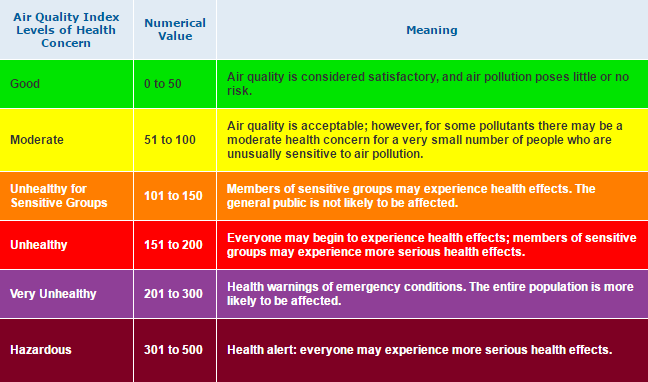
\includegraphics[width= 15 cm]{111.jpg}
	\caption{Air Quality Index}
\end{figure}





  %\ref for the figure label, check the below figure.

%%%%%%%%%%%%%%%%%%%%%%%%%%%%%%%%%%%
%		Before using image put the jpg image file in the folder. 
%		Here   ct.jpg   is the file name
%%%%%%%%%%%%%%%%%%%%%%%%%%%%%%%%%%%

\chapter{FEATURE SELECTION}  % Short of the project name

{\em A variety of meteorological, traffic and industrial parameters affect the air pollution level. After
taking consideration of the data availability and importance 5 Features are selected.}
\section{Data Overview}\
In order to identify and forecast key parameters affecting air quality and propose appropriate preventive strategies and policies, it is essential to systematically collect data characterizing air quality. The data includes two parts: training data set and test data set. Training data set has 322 observation points and the test data has 55 points. Each point represents the meteorological and traffic condition of a specific day in Beijing City. The total data set covers 47 days in 2014 and 330 days in 2013. The data comes from China Meteorological Data Sharing Service System, Beijing Transportation Research Center and US Embassy in Beijing. As mentioned before, the output data was labeled as one or zero. One refers to high pollution level and zero refers to low pollution level. The total number labeled as zero is 103, while the remaining 274 points are labeled as 0.
\pagebreak
\section{Parameters}
\begin{itemize}
\item{Temperature}

	\item{Wind Speed}

	\item{Relative Humidity}
	
	\item{Traffic Index}
	
	\item{Air Quality Of Previous Day}
	
	
\end{itemize}
\subsection{Temperature}

Temperature affect air quality because of temperate inversion: the warm air above cooler air acts like a lid, suppressing vertical mixing and trapping the cooler air at the surface. As pollutants from vehicles, fireplaces, and industry are emitted into the air, the inversion traps these pollutants near the ground.


\subsection{ Wind Speed}
Wind speed plays a big role in diluting pollutants. Generally, strong winds disperse pollutants, whereas light winds generally result in stagnant conditions allowing pollutants to build up over an area.

\subsection{ Relative Humidity}

Humidity could affect the diffusion of contaminant.

\subsection{ Traffic Index}
The large number of cars on the road cause high level of air pollution and traffic jam may increase the pollutants concentration from vehicles. The definition of traffic index is a index reflecting the smooth status of traffic. The index range is from 0 to 10. 0 represents smooth and 10 represents sever traffic jam.


\subsection{Air Quality Of Previous Day }
The air pollution level is influenced by the condition of the previous day to some extent. If the air pollution level of the previous day is high, the pollutants may stay and affect the following day.

\begin{figure}[h]
	\label{ss}    %Figure Label is used
	\centering
	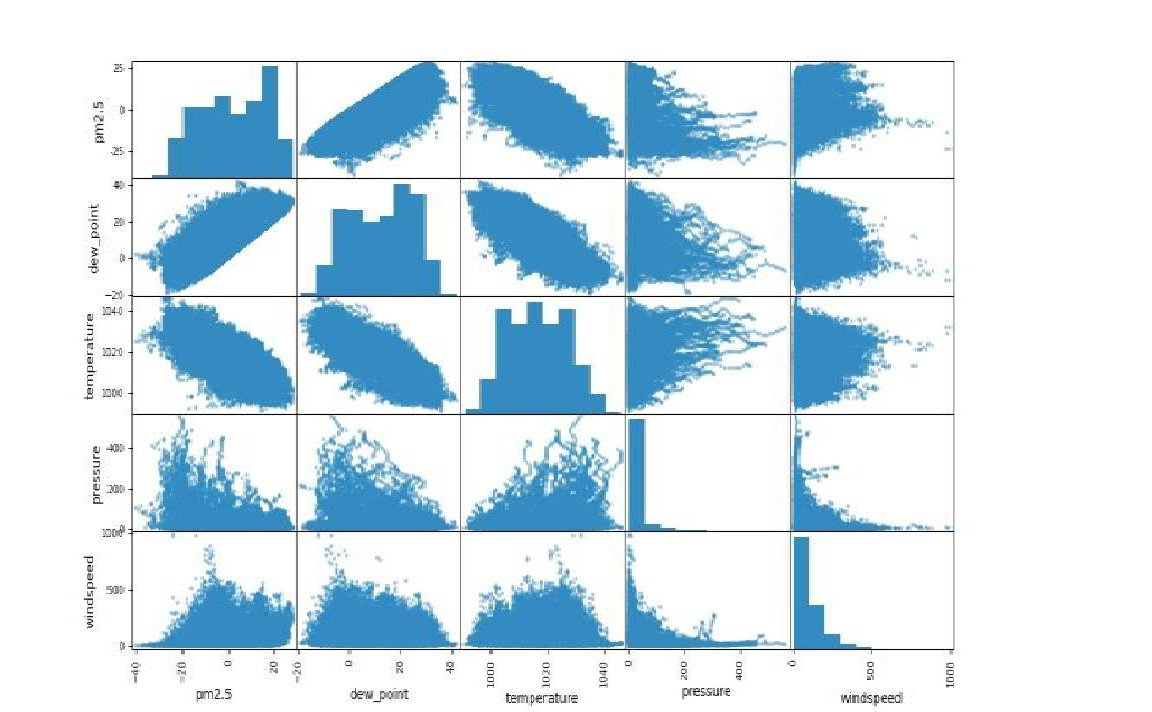
\includegraphics[width= 15 cm]{2.jpg}
	\caption{Scatter plot for the relation among attributes}
\end{figure}

\pagebreak
\chapter{METHODOLOGY}

\section{Two primary Phases }

\subsection{Training}

Estimating the parameters for the machine learning is called training the data. The observations in the training set form the experience that the algorithm uses to learn. In supervised learning problems, each observation consists of an observed output variable and one or more observed input variables.

\subsection{Testing}

Evaluating how well the machine learning method work is called testing. The test set is a set of observations used to evaluate the performance of the model using some performance metric. It is important that no observations from the training set are included in the test set. If the test 
set does contain examples from the training set, it will be difficult to assess whether the algorithm has learned to generalize from the training set or has simply memorized it.
\pagebreak
\section{Supervised Learning Algorithms}
This prediction is a binary classification problem, so the following three supervised learning algorithms were used:

\begin{itemize}
\item{Logistic Regression}

	\item{Naive Bayes Classification}

	\item{Support Vector Machines}
	
\end{itemize}

\subsection{Logistic Regression }
The output is a Generalized Linear Model. For this model, the prediction value is range for 0 to 1. In order to get the label, the values were converted to zero  and one. Logistic regression is the algorithm employed to detect a user-defined sample to be polluted or not. Logistic regression is the appropriate regression model to conduct analysis when the dependent variable is dichotomous. For example, here, the data set gets classified into two classes I.E, Polluted or Not Polluted. Like all regression analyses, the logistic regression is a predictive analysis. Logistic regression is used to explain the relationship between one or more independent variables and one dependent binary variable.


\begin{figure}[h]
	\label{ss}    %Figure Label is used
	\centering
	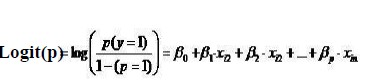
\includegraphics[width= 11 cm]{3.jpg}
	\caption{Logit Function}
\end{figure}

Logit function is used to generate log odds of an attribute that signifies the probability of the attribute. Log odds are an alternate way of expressing probabilities, which simplifies the process of updating them with new evidence.
Based on logit function, the system classifies the training data to be either 0 (not polluted) or 1 (polluted) and verifies its accuracy using the test data. The result of the user input is also 0/1 and not the PM2.5 level



\subsection{Naive Bayes Classification}

The Naive Bayes Classifier technique is based on the so-called Bayesian theorem and is particularly suited when the dimensionality of the inputs is high. Despite its simplicity, Naive Bayes can often outperform more sophisticated classification methods.

\begin{figure}[h]
	\label{ss}    %Figure Label is used
	\centering
	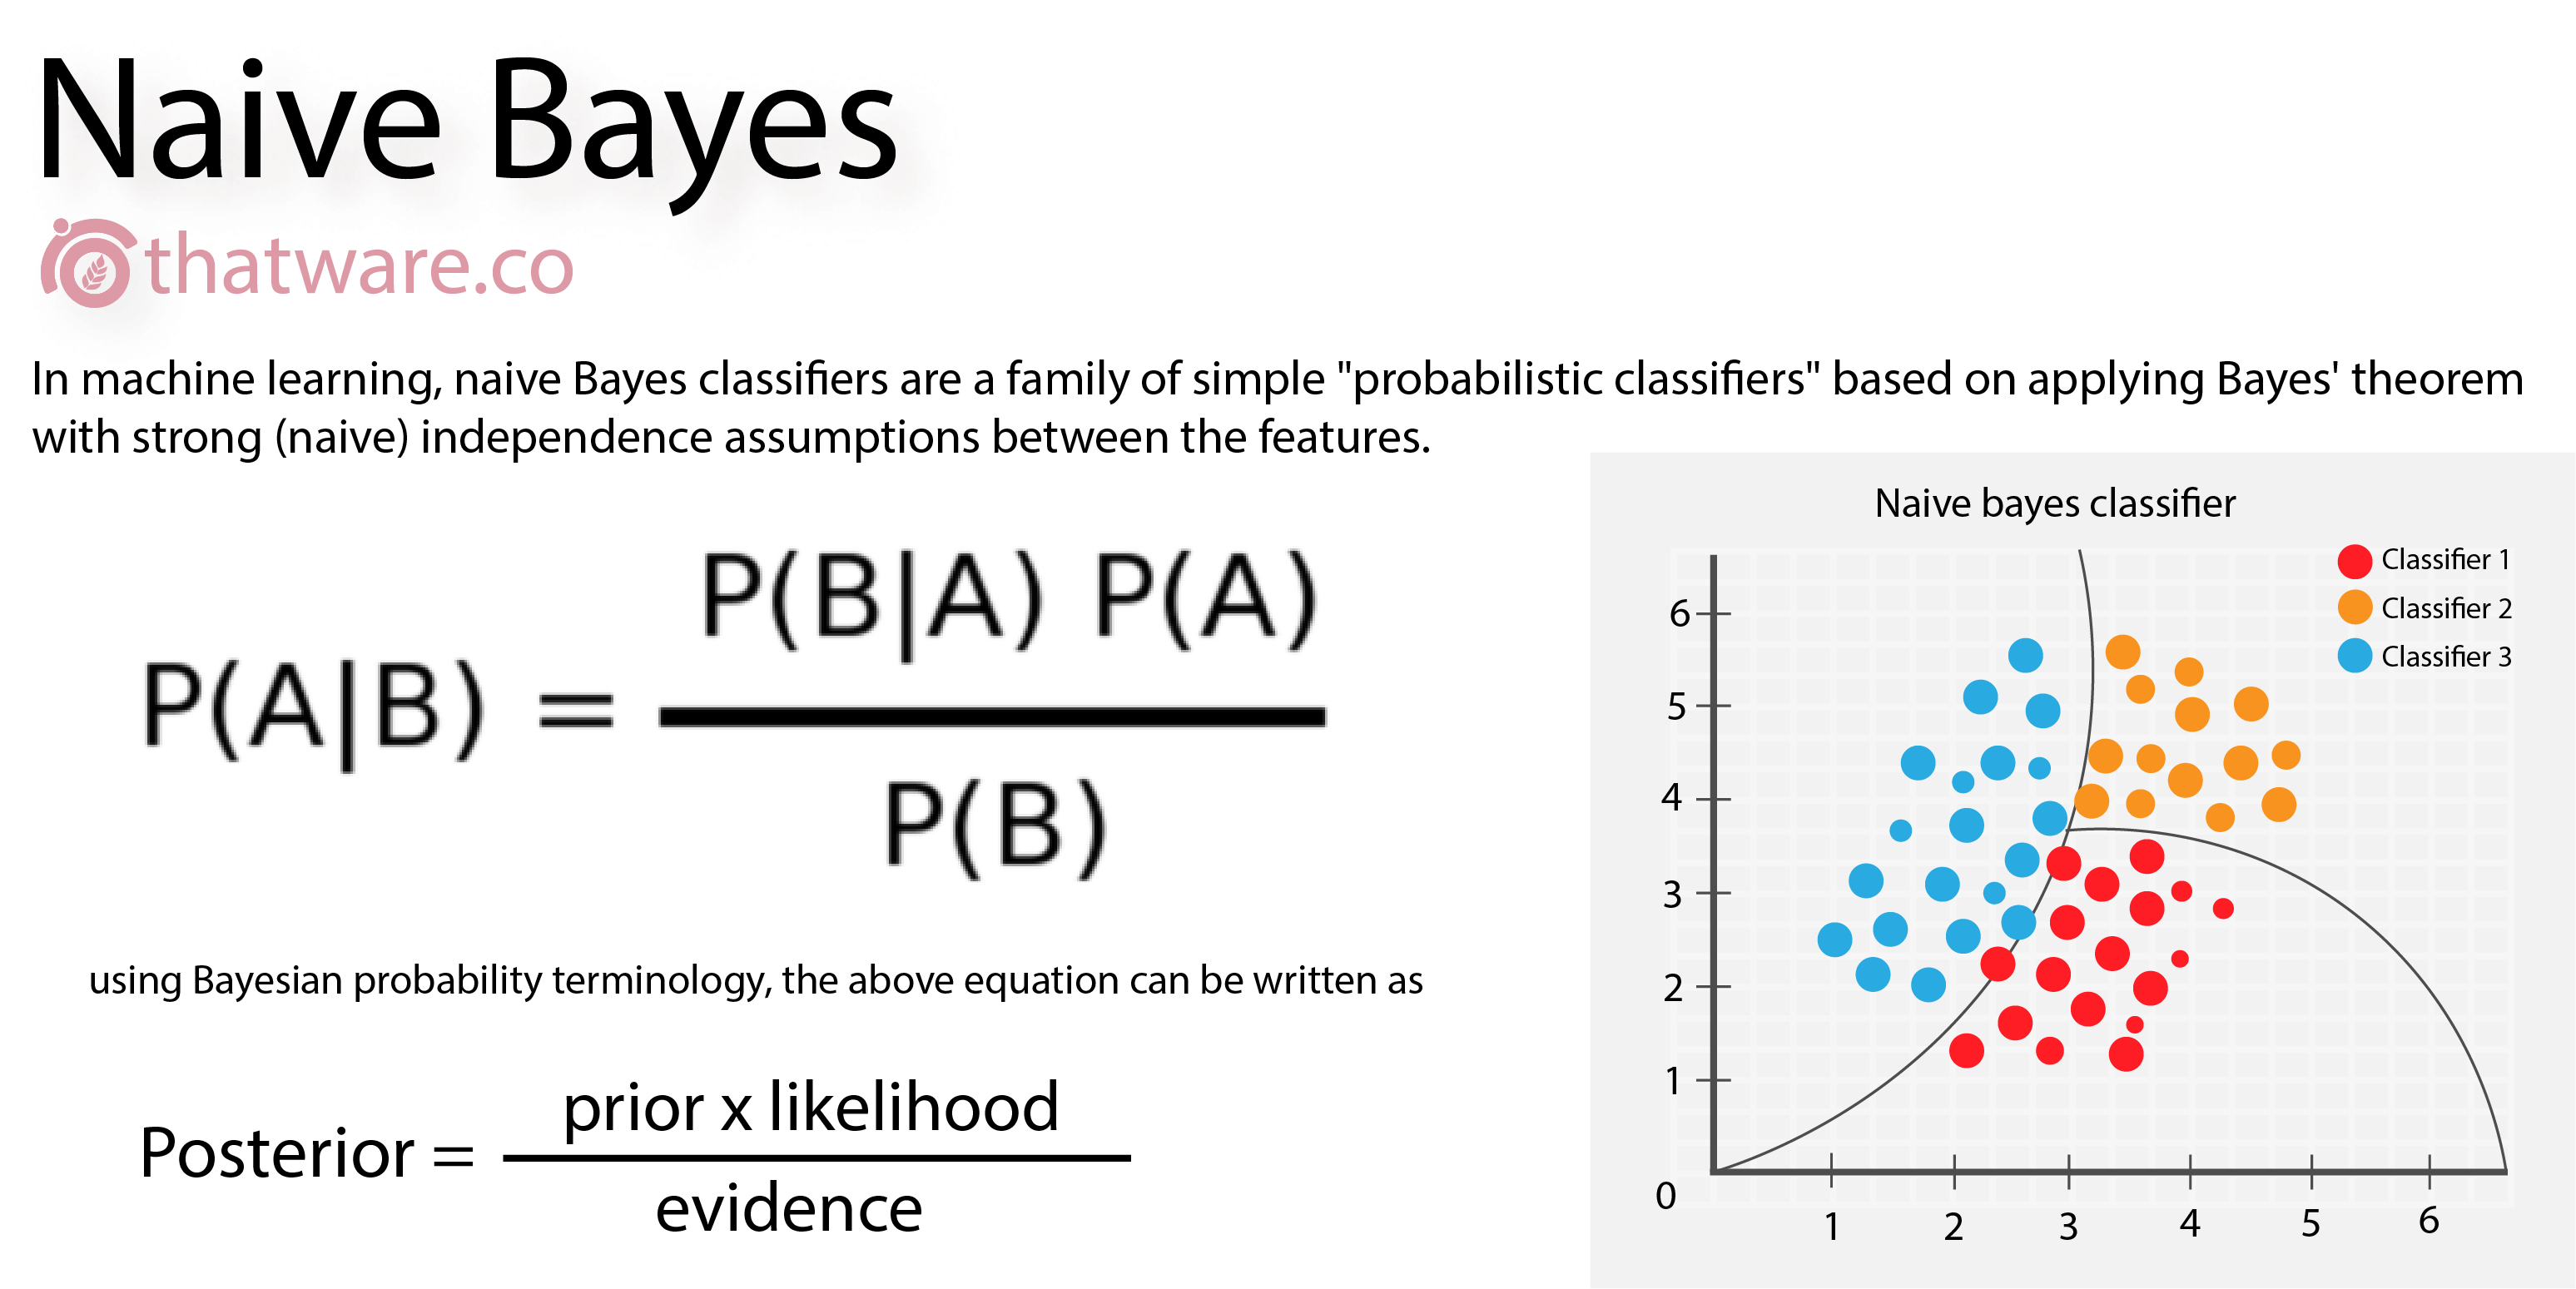
\includegraphics[width= 15 cm]{4.jpg}
	\caption{Naive Bayes Classifier }
\end{figure}

 Naive Bayes classifiers can handle an arbitrary number of independent variables whether continuous or categorical. Given a set of variables, X = {x1,x2,x...,xd}, we want to construct the posterior probability for the event Cj among a set of possible outcomes C = {c1,c2,c...,cd}. In a more familiar language, X is the predictors and C is the set of categorical levels present in the dependent variable. Using Bayes' rule:
\begin{figure}[h]
	\label{ss}    %Figure Label is used
	\centering
	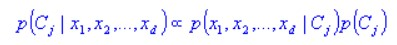
\includegraphics[width= 15 cm]{bayers1.jpg}
	\caption{Bayes rule  }
\end{figure}

where p(Cj | x1,x2,x...,xd) is the posterior probability of class membership, i.e., the probability that X belongs to Cj. Since Naive Bayes assumes that the conditional probabilities of the independent variables are statistically independent we can decompose the likelihood to a product of terms:

\begin{figure}[h]
	\label{ss}    %Figure Label is used
	\centering
	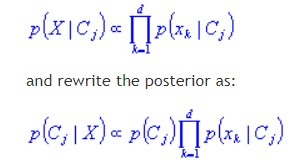
\includegraphics[width= 11 cm]{bayers2.jpg}
	\caption{Bayes rule }
\end{figure}

\pagebreak

\subsection{Support Vector Machine}


Support Vector Machine(SVM) is a supervised machine learning algorithm which can be used for both classification or regression challenges. However,  it is mostly used in classification problems. In this algorithm, plot each data item as a point in n-dimensional space (where n is number of features you have) with the value of each feature being the value of a particular coordinate. Then, we perform classification by finding the hyper-plane that differentiate the two classes very well 


\begin{figure}[h]
	\label{ss}    %Figure Label is used
	\centering
	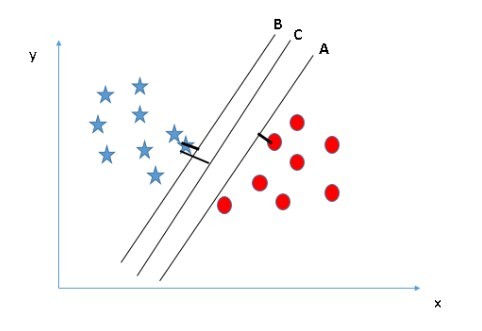
\includegraphics[width= 11 cm]{svm1.jpg}
	\caption{Support Vector Machine }
\end{figure}	

The main objective in SVM is to find the optimal hyperplane to correctly classify between data points of different classes (Figure 2). The hyperplane dimensionality is equal to the number of input features minus one (eg. when working with three feature the hyperplane will be a two-dimensional plane).

\begin{figure}[h]
	\label{ss}    %Figure Label is used
	\centering
	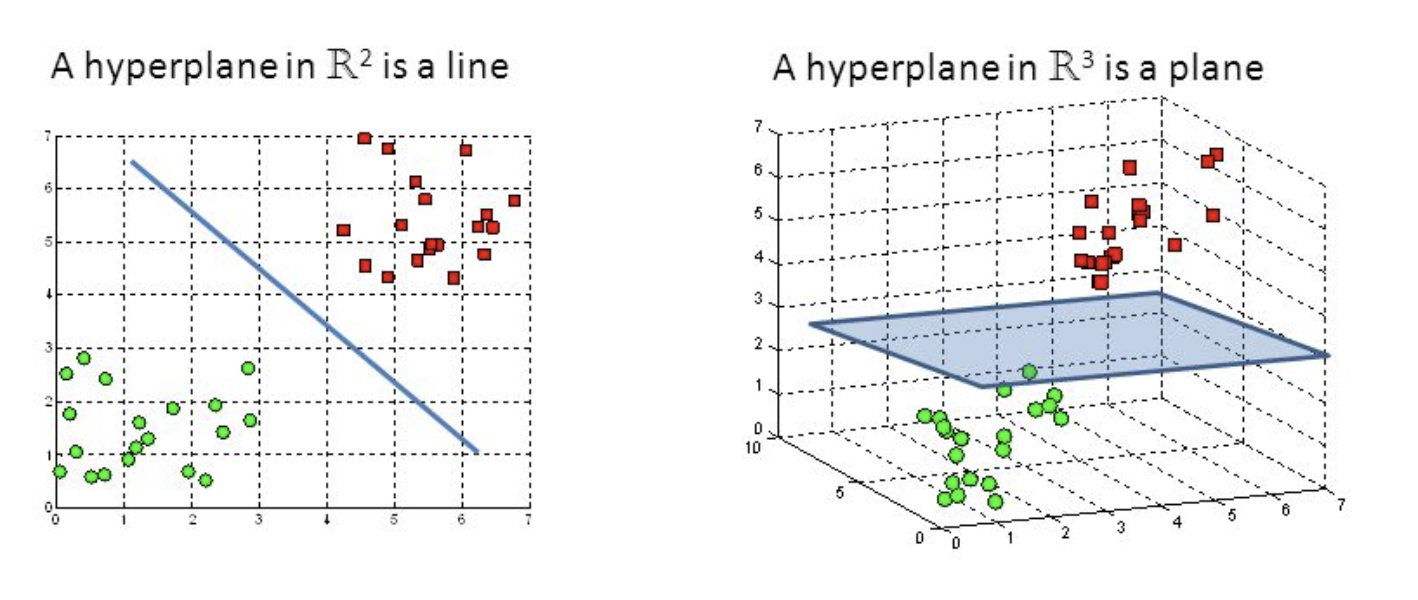
\includegraphics[width= 11 cm]{svm2.png}
	\caption{Hyper Plane in R2 and R3 }
\end{figure}	
 Data points on one side of the hyperplane will be classified to a certain class while data points on the other side of the hyperplane will be classified to a different class. The distance between the hyperplane and the first point (for all the different classes) on either side of the hyperplane is a measure of sure the algorithm is about its classification decision. The bigger the distance and the more confident we can be SVM is making the right decision. The data points closest to the hyperplane are called Support Vectors. 
 

\section{Result Analysis}

\begin{figure}[h]
	\label{ss}    %Figure Label is used
	\centering
	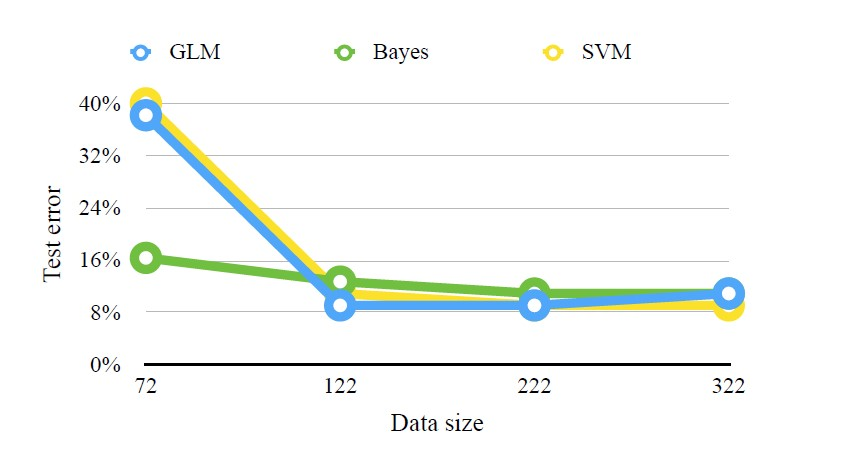
\includegraphics[width= 09 cm]{erroranaly.jpg}
	\caption{Algorithm Comparison }
\end{figure}	
When compared to other machine learning models applied on the data set. The overall test error for Logistic regression is 10.91, which is the same as it for
Bayes. SVM has the lowest test error, 9.09. After changing the data size and repeat training the model the test error of Bayes classifier doesn’t change much
with data size, however Logistic regression and SVM have large test error change with data size. Further more, the test error for SVM has the decline trend if the data size increases further.



\section{Performance Analysis}
the prediction of air pollution level with the ground data set, The best algorithm (SVM) gave the 0.722 precision, 1.000 recall and 0.839 FMeasure value. It is relatively accurate and is an acceptable result for practical use. However, compared with results from some literature, the predicting performance (F-Measure value) for this data set is not very good. Also, the advantage of SVM are not shown obviously.

\begin{figure}[h]
	\label{ss}    %Figure Label is used
	\centering
	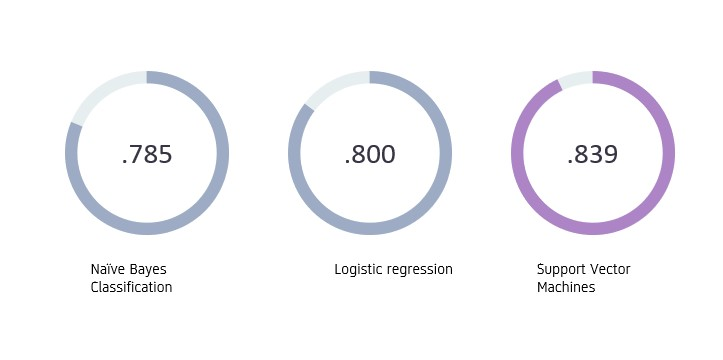
\includegraphics[width= 11 cm]{8.jpg}
	\caption{Performance Analysis(F-measure) }
\end{figure}	

\chapter{NEW PROPOSAL}

The data set in this project is not large enough. Air quality is a long-term formed problem and it is better to use a large data covering a variety of years and locations. Furthermore, beside the meteorological and traffic factors, industrial parameters such as power plant emissions also play significant roles in air pollution. Using Extreme Gradient Boosting(Egbooster) Or Auto regression Algorithm  Can make More accurate prediction over Support vector machine


\section{Autoregression}

Autoregressive models and processes are stochastic calculations in which future values are estimated based on a weighted sum of past values. Autoregressive models and processes operate under the premise that past values have an effect on current values, which makes the statistical technique popular for analyzing nature, economics, and other time-varying processes. Multiple regression models forecast a variable using a linear combination of predictors, whereas autoregressive models use a combination of past values of the variable.

\begin{figure}[h]
	\label{ss}    %Figure Label is used
	\centering
	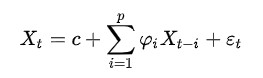
\includegraphics[width= 11 cm]{9.jpg}
	\caption{ Equation of AR }
\end{figure}	


\section{Extreme Gradient Boosting}

XGBoost is an optimized distributed gradient boosting library designed to be highly efficient, flexible and portable. It implements machine learning algorithms under the Gradient Boosting framework. XGBoost provides a parallel tree boosting that solve many data science problems in a fast and accurate way. 


\begin{figure}[h]
	\label{ss}    %Figure Label is used
	\centering
	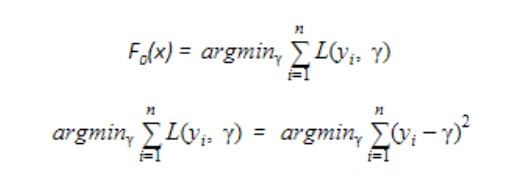
\includegraphics[width= 11 cm]{10.jpg}
	\caption{ Equation of XGBoost }
\end{figure}	

\chapter{CONCLUSION}

The regulation of air pollutant levels is rapidly becoming one of the most important tasks. It is important that people know what the level of pollution in their surroundings is and takes a step towards fighting against it. The results show that machine learning models (logistic regression and autoregression) can be efficiently used to detect the quality of air and predict the level of PM2.5 in the future. The proposed system will help common people as well as those in the meteorological department to detect and predict pollution levels and take the necessary action in accordance with that. Also, this will help people establish a data source for small localities which are usually left out in comparison to the large cities.


%%%%%%%%%%%%%%%%%%%%%%%%%%%%%%%%
%%%%%%%%%%%%%%%%%%%%%%%%%%%%%%%%
%%%%%%%%%%%%%%%%%%%%%%%%%%%%%%%%
\clearpage
%%%%%%%%%%%%%%%%%%%%%%%%%%%%%%%%


%%%%%%%%%%%%%%%%%%%%%%%%%%%%%%%%%%%%
%%%%%%%%%%%%%%%%%%%%%%%%%%%%%%%%%%%%
%%
%%          Bibliography 
%%
%%%%%%%%%%%%%%%%%%%%%%%%%%%%%%%%%%%%
%%%%%%%%%%%%%%%%%%%%%%%%%%%%%%%%%%%%

\clearpage
\addcontentsline{toc}{chapter}{\quad BIBLIOGRAPHY}
\begin{thebibliography}{99}
	%%%%%%%%%%%%%%%%%%%%%%%%%%%%%%%%%%%%
	%%
	%%          Add Bibliography from below, here 3 eg are there
	%%	    If u need to add more bib  use \bibitem   command again & again
	%%
	%%%%%%%%%%%%%%%%%%%%%%%%%%%%%%%%%%%%
	
\bibitem{a}Dan wei: Predicting air pollution level in a specific city [2014]
\bibitem{b}Pandey, Gaurav, Bin Zhang, and Le Jian. quot; Predicting sub-micron air pollution indicators: a machine learning approach.quot ; Environmental Science: Processes  amp; Impacts 15.5 (2013): 996-1005.
\bibitem{c}Athanasiadis, Ioannis N., et al. "Applying machine learning techniques on air quality data for real-time decision support." First international NAISO symposium on information technologies in environmental engineering (ITEE'2003), Gdansk, Poland. 2003.
\bibitem{d}Aditya C R, Chandana R Deshmukh, Nayana D K, Praveen Gandhi Vidyavastu:Detection and Prediction of Air Pollution using Machine Learning Models
\bibitem{e}https://en.wikipedia.org/wiki/Support-vector machine
\bibitem{f}https://en.wikipedia.org/wiki/Logistic regression
\bibitem{g}https://en.wikipedia.org/wiki/Particulates
\bibitem{h}https://towardsdatascience.com/naive-bayes-classifier-81d512f50a7c
\bibitem{i}https://machinelearningmastery.com/logistic-regression-for-machine-learning/
\bibitem{j}https://www.analyticsvidhya.com/blog/2017/09/understaing-support-vector-machine-example-code/
\bibitem{k}https://en.wikipedia.org/wiki/Naive Bayes classifier

	
	
	








	
\end{thebibliography}



%%%%%%%%%%%%%%%%%%%%%%%%%%%%%%%%%%%%%
%%%%%%%%%%%%%%%%%%%%%%%%%%%%%%%%%%%%%
\clearpage




%%%%%%%%%%%%%%%%%%%%%%%%%%%%%%%%%%%%%
%%%%%%%%%%%%%%%%%%%%%%%%%%%%%%%%%%%%%
%
%   Hi, All
%   Arun Xavier, VAST Thrissur
%
%   for more  Visit my Page - http://arunxeee.blogspot.in/
%
%%%%%%%%%%%%%%%%%%%%%%%%%%%%%%%%%%%%
%%%%%%%%%%%%%%%%%%%%%%%%%%%%%%%%%%%%

%
\end{spacing}
\newpage
\thispagestyle{empty}
\vspace*{\fill}
\begin{flushright}

\includegraphics[width=2.5 cm]{VidyaLogo.JPG}\\[.2 cm]
{\Large \bf \rm  Department of \vdept\ }\\
{\large \rm Vidya Academy of Science \& Technology\\
Thalakkottukara, Thrissur - 680 501\\
({\tt http://www.vidyaacademy.ac.in})}
\end{flushright}

%
\end{document}